Particle detectors produce timeseries data of electrical signals corresponding to particle interactions, which coupled with precision knowledge of detector geometry can be used to reconstruct individual particles' momenta, which can then provide complete records of entire events. An example event is shown in \figref{fig:example-track}, illustrating detector hits and the corresponding reconstructed particle paths.

\begin{figure}[htb]
    \centering
    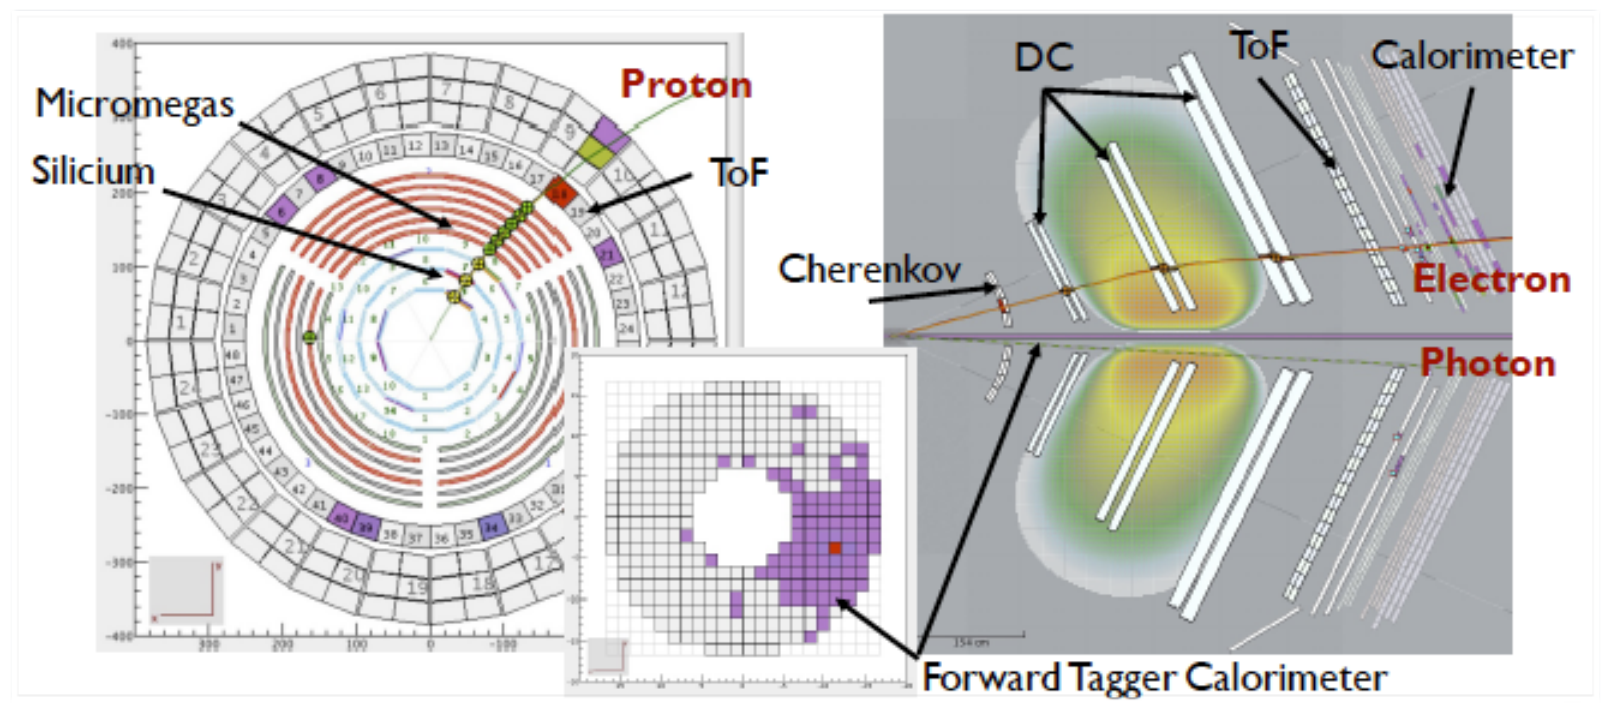
\includegraphics[width=0.9\textwidth]{Chapters/Ch2-Experiment/recon_pid/pid_figs/example_track.png}
    \caption[Example Event Tracks]{Track showing an example path of an electron, proton, and photon, from \parencite{Battaglieri2021PresentProgram}.}
    \label{fig:example-track}
\end{figure}


\subsection{Decoding and Track Reconstruction}\label{sec:decoding_reconstruction}
    The timeseries data from the detector systems must be efficiently processed and stored for future analysis. The data acquisition system (DAQ) was originally designed to handle a 10 kHz event rate and 100 MB/s event rate, but has since been shown to be able to handle event rates of 30 kHz at data rates above 1 GB/s \parencite{Boyarinov2020TheSystem}.  The CLAS12 system consists of more than 100k individual readout channels and utilizes 250 MHz FADCs to digitize signals. Data for this analysis utilized an inclusive electron trigger requiring electron momentum p$_{\mathrm{e'}}$ above 2 GeV/c \parencite{Raydo2020TheSystem}. The raw detector hits are organized into into tabular structures called ``banks'' and are subsequently passed to the CLAS12 Reconstruction and Analysis Framework (CLARA) \parencite{Gyurgyan2016CLARA:Framework}.

    Detector hits in each event are converted into particle tracks through hit clustering, pattern matching, and Kalman filter algorithms. The momentum \textit{p} of a particle with charge \textit{q} is related to its track through a magnetic field by \eqref{eq:particle_track},
    
    \begin{equation}\label{eq:particle_track}
        \frac{q}{p} = \frac{\Delta \theta}{c \int B dl},
    \end{equation}

    where $\Delta \theta$ is the deflection angle of the curve, \textit{c} is the speed of light, and $\int B dl$ is the line-integrated magnetic field along the track. Charge parity (positive or negative) is determined from the deflection direction (e.g. negative particles bend away from the beamline when the torus has value ``outbending''). Time-of-flight detectors provide a direct measure of particle speed $\beta = \frac{v}{c}$, which,when coupled with track information yields the complete charged particle information. This analysis is only concerned with proton and electron identification, but \figref{fig:clas12-pid-overview} details particle discrimination across different detectors and energy regimes.
    
    Photons are identified from their depositions in the ECal and lack of interactions in the DCs. Events undergo this analysis process (``cooking'') and are stored as Event I/O (EVIO) files \parencite{Wolin2007EVIOPackage}, a format commonly used across JLab. The CLAS collaboration converts these files into High Performance Output (HIPO) format files \parencite{Ziegler2020TheReconstruction}, which has more optimized functionality for the CLAS software packages. 

    \begin{figure}[H]
        \centering
         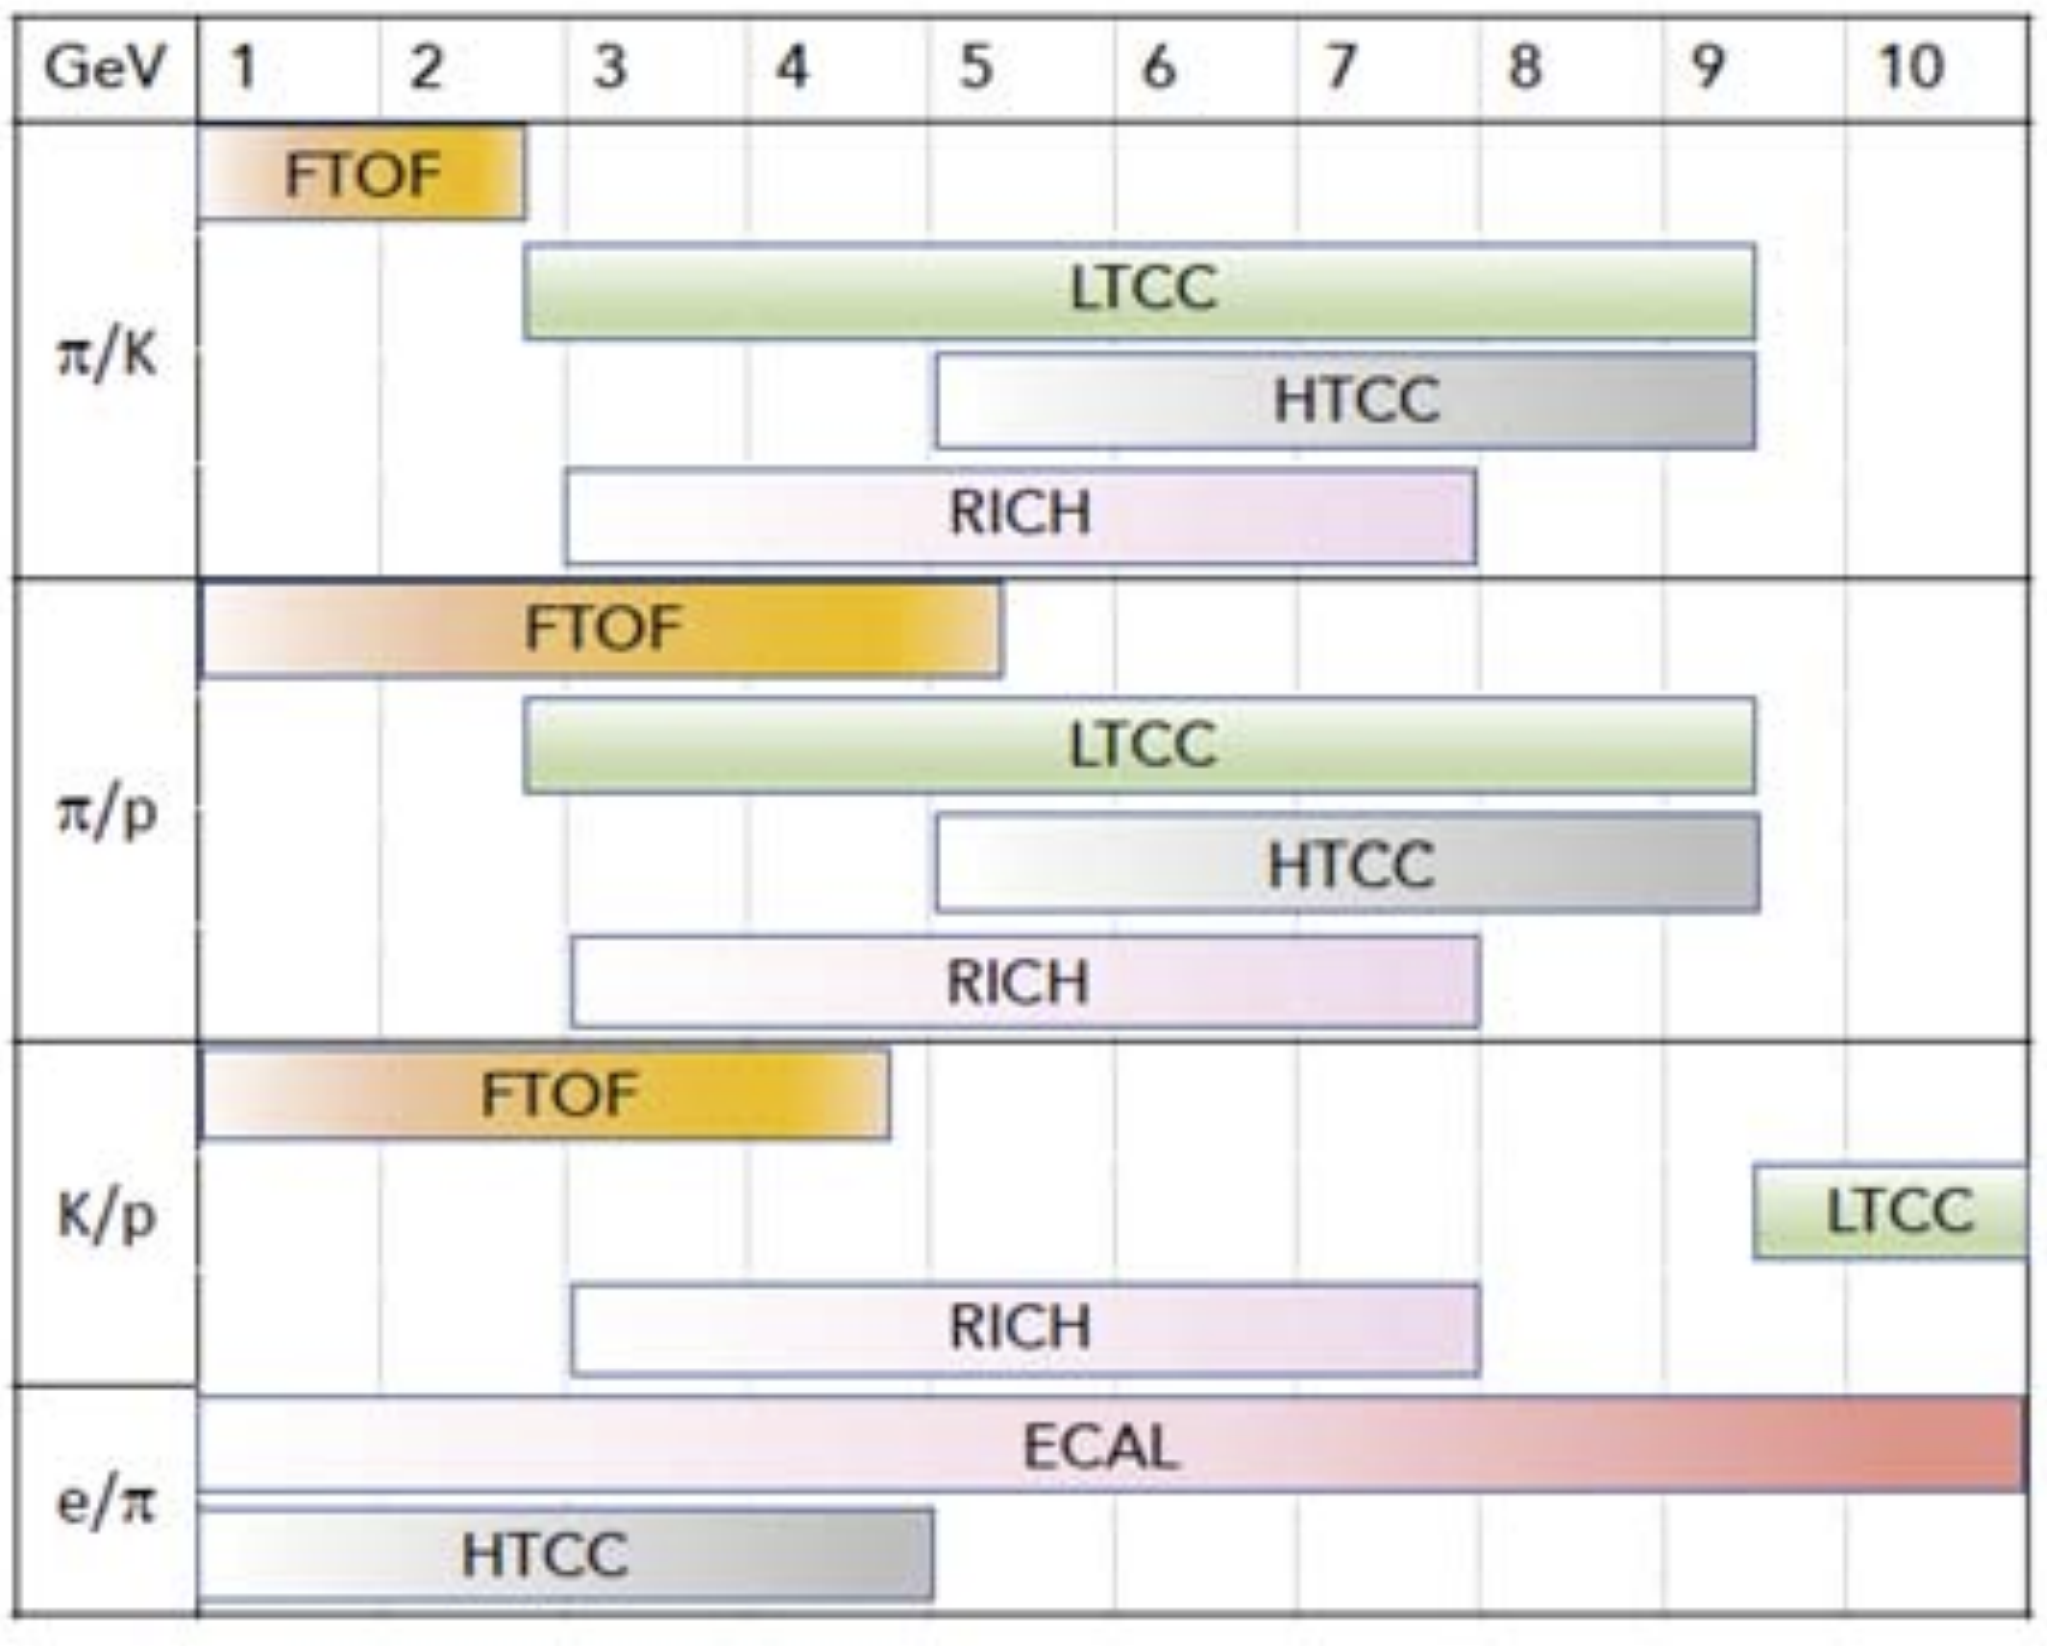
\includegraphics[width=0.5\textwidth]{Chapters/Ch2-Experiment/recon_pid/pid_figs/pid-clas12-new.png}
        \caption[Particle Separation by Detector]{Map detailing how different detectors are able to separate particle species across different energy regimes. Color intensity is scaled to separation sensitivity (more intense color equates to higher sensitivity). From \parencite{Burkert2020TheLaboratory}.}
        \label{fig:clas12-pid-overview}
    \end{figure}


    \iffalse
    should maybe include some beta vs p curves

    \fi
\subsection{Particle Identification}\label{sec:pid}
    The final state for the \dvpip process is an electron, a proton, and a neutral pion, which promptly decays into two photons. This work requires full final state detection for event selection, so all three particles must be well reconstructed. Further, the neutral pion must be identifiable from the photon four-momenta. Basic, conservative particle identification is performed in data cooking (``event builder cuts''), from which point additional modifications corresponding to known detector dead regions, inefficiencies, and reconstruction issues are added. A set of modifications common to all efforts analyzing this data set is known as the ``\href{https://www.overleaf.com/project/5ea737720942930001ff5e9c}{RG-A common analysis cuts}''. For this analysis, electrons are identified in the FD, the CD and FD are utilized for proton tracks, and the FT and FD are used for photon identification. The main utility of each detector sub-system is summarized in \tabref{tab:detector_components}.
 
    \begin{table}[htb]
        \centering
        \begin{tabular}{c|c|c}
            System & Detector  & Utility in this Analysis \\
            \hline
            \multirow{6}{*}{FD} & HTCC & $\mathrm{e'}$ trigger, PID \\
            & FTOF & $\mathrm{e'}$ trigger, $\mathrm{p'}$ PID \\
            & DC & $\mathrm{e'}$ trigger, $\mathrm{e'}$ and $\mathrm{p'}$ momentum \\
            & ECAL & $\mathrm{e'}$ trigger, PID, $\gamma$ energy, $\pi^0$ angle \\
            & \textcolor{gray}{LTCC} & \textcolor{gray}{not used} \\
            & \textcolor{gray}{RICH} & \textcolor{gray}{not used} \\
            \hline
            \multirow{5}{*}{CD} & CTOF & $\mathrm{p'}$ PID \\
            & CVT & $\mathrm{p'}$ momentum \\
            & \textcolor{gray}{CND} & \textcolor{gray}{not used (LH2 target)} \\
            & \textcolor{gray}{FMT} & \textcolor{gray}{not installed} \\
            & \textcolor{gray}{BAND} & \textcolor{gray}{not installed} \\
            \hline
            \multirow{3}{*}{FT} & FT-Hodo & $\gamma$ PID \\
            & FT-Cal & $\gamma$ energy \\
            & FT-Trk & $\gamma$ angle \\
        \end{tabular}
        \caption[CLAS12 Detectors Main Functions]{Description of the components of the CLAS12 detector system and their primary usage in this work. Modified from \parencite{Lee2022MeasurementDetector}.}
        \label{tab:detector_components}
    \end{table}

    \subsubsection*{Electron}
        Electrons' light mass (510.9989 keV/c$^2$) and negative charge allows for relatively straightforward identification compared to hadrons. Conditions applied at the Event builder level include: $\beta \sim 1$ at all momenta, track curve consistent with a negatively charged particle, and a cut of the number of photoelectrons produced in the HTCC to differentiate it from $\pi^-$ particles. Above 5 GeV/c$2$, electrons are differentiated from negative pions by the sampling fraction (SF) in the calorimeters. Additional fiducial cuts were included to require the reconstructed electron track vertex along the beamline, $v_{z_{e'}}$ to fall within the -5.5 cm to -0.5cm nominal target location in the CLAS12 coordinate system, which is conservatively implemented as falling within a (-13,12) or (-18,10) cm range, for the inbending and outbending configurations, respectively. 
        
    

    
    \subsubsection*{Proton}
        Proton identification is achieved primarily through $\beta$ vs \textit{p} curves as previously discussed and as shown in \figref{fig:clas12-pid-overview}. Sangbaek Lee, a collaborator working on another deeply virtual process, DVCS, developed additional fiducial cuts for the central detector region based on requiring 3$\sigma$ limits on the difference between proton and electron interaction vertices locations ($v_{z_{e'}} - v_{z_{p'}}$) as well as 3$\sigma$ limits on the difference between measured time of flight and a track-reconstruction based ToF calculation, as detailed in \parencite{Lee2022MeasurementDetector}.

    
    \subsubsection*{Photon}
        Photons are primarily identified by a lack of DC tracks along with ECal hit clusters totaling more than 400 MeV. A real photon has speed $\beta=1$, but a conserative threshold is allowed of $0.9<\beta<1.1$ to rule out neutrons that can form from nuclear reactions. Fiducial cuts are employed in congruence with RG-A common analysis efforts. 
    
    %    **photon cuts:
     %   pid 22, status > 2000 (in FD or CD, not ftagger)
      %  momentum greater than 400 MeV each
        
    \subsubsection*{Neutral Pion}
        In addition to individual particle identifications procedures for photons, neutral pions are identified by calculating the invariant mass between two photons. If an event has more than two photons, all possible permutations are calculated to identify possible $\pi^0$ candidates, which are classified as having a mass close to the known mass of 134.977 MeV/c$^2$. This identification, combined with cuts on missing mass and momentum as discussed in section \ref{sec:eventselection} yield the pion distribution shown in \figref{fig:combined_pion_fig}. 
        
        \begin{figure}[hbt]
            \centering
            \subfloat[The distribution for mass of two photons $M_{\gamma\gamma}$.]{\label{fig:ggmass}\includegraphics[page=6,width=0.45\textwidth]{Chapters/Ch2-Experiment/recon_pid/pid_figs/eppi0.exclusive.pdf}}\hfill
            \subfloat[The distribution for mass of two photons after exclusivity cuts.]{\label{fig:ggmass_after}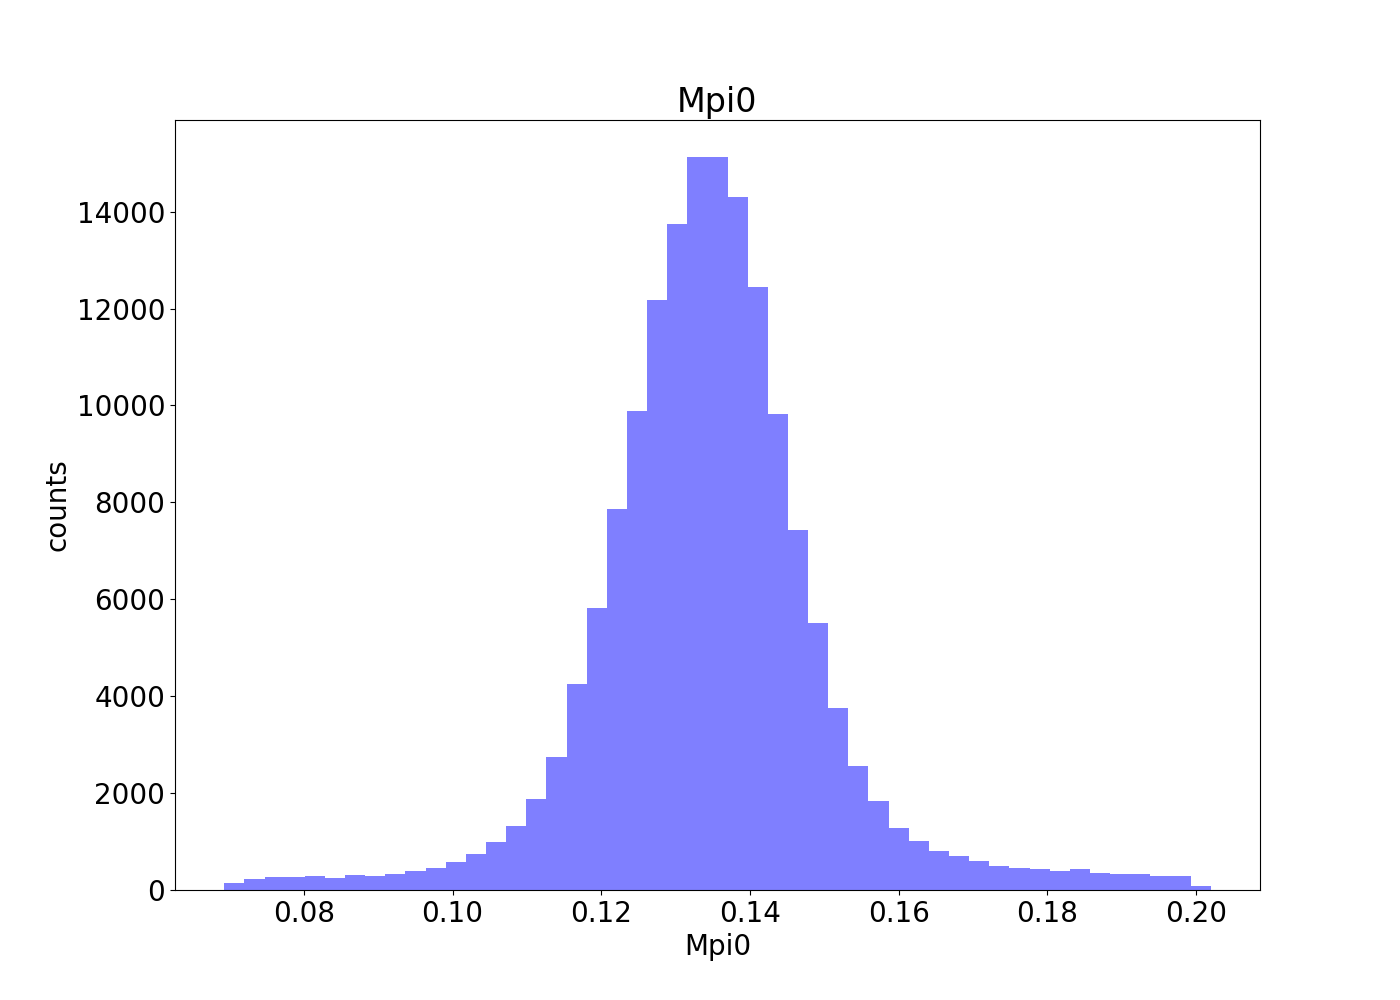
\includegraphics[width=0.45\textwidth]{Chapters/Ch2-Experiment/recon_pid/pid_figs/Mpi0.png}}
            \caption[$\gamma \gamma$ Invariant Mass Distribution]{$\gamma \gamma$ invariant mass distribution before (a) and after (b) exclusivity cuts.}
            \label{fig:combined_pion_fig}
        \end{figure}
            


\subsection{Data Storage and Formatting}\label{sec:filtering}
    The raw, trigger inclusive dataset for just this data taking run (Fall 2018) occupies O(1 PB) of disk space, which is too cumbersome for direct analysis. Data is ``skimmed'', which involves using very loose cuts to throw out trigger events that have a very low probability of being of interest. This process produces ``trains'' (also called ``wagons'') which are smaller size O(100 GB) datafiles that are amenable to analysis processing. In this analysis, events were considered that included loose PID requirements to contain one electron, one proton, and at least two photons.  These HIPO files are readily available through JLab's scientific computing nodes. 

    
    For the ease of applicability of several existing software utilities \parencite{Virtanen2020SciPyPython}, \parencite{Harris2020ArrayNumPy}, these files are converted to other data formats before final analysis. In particular, the HIPO files are passed through the PID cuts discussed above in a process known as filtering \parencite{Lee2023FilterEvents} and converted using CLAS12ROOT \parencite{Glazier2023Clas12root} into the popular nuclear and particle physics data format known as ROOT \parencite{Brun1997ROOTFramework}. These files are then further converted using UPROOT \parencite{Pivarski2022Scikit-hep/uproot4:4.2.1} to a pickle format \parencite{Python2023PickleSerialization}, which is a serialized, space efficient data object that is standard in the Python library system. The pickled files are saved for short term storage and passed to structures to compute the process cross section, as discussed in chapter \ref{Chapter:BaseAnalysis}. \figref{fig:DataReductionPipeline} illustrates this data processing chain, resulting in $\sim$ 1 GB of experimental events from many terabytes of initial reconstructed event data. The simulated data (Ch. \ref{Chapter:Simulations}) is passed through the same processing chain with similar disk attrition ratios, at which point the \xsec can be calculated (Ch. \ref{Chapter:BaseAnalysis}). 

        
    \begin{figure}
        \centering
        \begin{tikzpicture}[auto, node distance=0.5cm, inner sep=1pt,
        box/.style={rectangle, draw, minimum size=#1, align=center}]
            \node [box=15cm, fill=burgundy] (cooked) {};
            \node [anchor=north, yshift=-0.5cm, text=white] at (cooked.north) {\textbf{\textcolor{white}{Cooked HIPO files - 51,000 GB}}};
            \node [box=11.8cm, fill=britishracinggreen, inner sep=0.4cm] (filtered) at (cooked.center) {};
            \node [anchor=north, yshift=-0.5cm, text=white] at (filtered.north) {\textbf{\textcolor{white}{Skimmed HIPO trains - 4,000 GB}}};
            \node [box=3.35cm, fill=darkblue, inner sep=0.4cm] (events) at (filtered.center) {};
            \node [anchor=north, yshift=-0.3cm, text=white] at (events.north) {\textbf{\textcolor{white}{Uproot - 5 GB}}};
            \node [box=1cm, fill=mypurp, inner sep=0.4cm] (dvip) at (events.center) {};
            \node [anchor=north, yshift=-0.5cm, text=white] at (dvip.north) {\textbf{\textcolor{white}{\tiny{1 GB}}}};
        \end{tikzpicture}
         \caption[Data Processing Pipeline]{Size reduction in the data preparation pipeline for the Fall 2018 dataset (configurations combined). The box heights correspond to the logarithm of total data size at that processing step. The smallest box is the approximate size of the final file containing all \dvpip events, more details can be found in Chapter \ref{Chapter:BaseAnalysis}.}
         \label{fig:DataReductionPipeline}
    \end{figure}


    \iffalse
    
    \subsubsection*{Data Location and Availability}
        Data is stored accessible on ifarm, with trains
        
    \subsubsection*{File Formatting and Conversion}\label{sec:filtering}
        Mention that same transformations are used for rec events and filtering
        hipo to root to uproot

    \fi
    




\iffalse
%FROM SANGBAEK
During RG-A data taking, the event was triggered in parallel by three physics trigger systems: (1) the electron trigger, (2) photoproduction trigger and (3) opposite sector trigger. This analysis focuses on the (inclusive) electron trigger that is designed to record events with FD electron candidates with minimum $n_{phe}$, $E_{dep.}$, $E_{dep.} PCAL$ conditions and the geometrical matching between detector subsystems. The electron trigger search was adjusted and performed in parallel for each sector. The electron trigger system is highly efficient with 99.5\% trigger efficiency and 95\% DAQ livetime for trigger electrons of momentum above 2 GeV/c. The desired event rate for the RG-A experiment is about 20 kHz, which was estimated using the simulation. This can be easily achieved by the CLAS12 trigger logic with the effective performance level up to 200 kHz \parencite{Raydo2020TheSystem}. The events triggered by the electron trigger has trigger bits ``1'' (True) in any of bits 0 to 6, where the bits 1–6 stan for each sector and 0 is their OR. The trigger bits can be accessed offline. Processing all saved inclusive events is not efficient in many aspects. There are a lot more inclusive events than the exclusive channels of interest, namely DVCS and DV$\pi^0$P. The RG-A has a few skimming modes, trains and wagons, to be commonly used for some specific channels. A train is a coarse skimming, such as the inclusive skim, which requires an electron-proton pair in one event. A wagon is a relatively finer skimming, such as the DVCS wagon, which requires one electron-proton-photon set with some level of DVCS exclusivity. The series of skimming processes is called data cooking. In this analysis, for the base data set we take the DVCS wagon that selects the DVCS candidates with loose exclusivity cuts, and require at least one $e'p'\gamma$ set in the event \textcolor{red}{158} (see Section 3.3 for the cut conditions). The raw data is stored in the HIPO format \textcolor{red}{151} for the entire CLAS collaboration. The HIPO format has the advantages of fast Input/Output (I/O) speed, and compatibility with the Event I/O (EVIO) format that is commonly used for the Jefferson Lab event storage  \parencite{Wolin2007EVIOPackage}. For this analysis, the python program with pandas library was taken as the main analysis tool in that python is supported by modern statistical packages \textcolor{red}{160,161} that are well maintained. This motivates operation of a custom pipeline to convert the data format to pickle, which is the python standard data format \textcolor{red}{162}. We use the CLAS12ROOT \textcolor{red}{163}, a software package to read the HIPO format in C++ and store the related information in ROOT format \textcolor{red}{164}. The ROOT formatted data is once again converted to pickle format, using the uproot library \textcolor{red}{165}. By doing so, the data are reduced into $M \times N$ dimensionality, where $M$ is the number of events, and $N$ is the number of physical quantities and other information that are related (Fig. 2-16). Different data formats have advantages in different stages of data processing. We filter the base data with the PID cuts introduced at Section 2.4 and save in another HIPO format, because the base data contains all detector responses. The filtered HIPO files are converted into ROOT format. Finally, we execute the python script to select DVCS and DV$\pi^0$P events with tighter Event Selection criteria that will be described at 3.3 and save them in the pickle format.

An electron candidate e'is defined as an associated signal of these FD signals: (1) a track in DC, (2) photoelectrons in HTCC, (3) hits in FTOF, (4) energy deposited over 60 MeV, and (5) the Sampling Fraction (SF) of Minimum Ionizing Particle’s (MIPs). Here, the event start time is determined from the track information, and corrected by the RF signal and the vertex location. The momentum of a charged particle such as e' and the proton p' is reconstructed using the equation of motion in a magnetic field. The polar angle difference during the trajectory $\Delta \theta$ is related to the momentum p and the charge q of the particle, and the line-integrated magnetic field along the trajectory curve, (int B dl) as

\begin{equation}
    \frac{q}{p} = \frac{\Delta \theta}{c \int B dl}
\end{equation}

During one event, p' is identified when there is a positively charged track in the DC
or the CVT, associated with FTOF or CTOF hits for the timing. The flight time $\Delta t_{p'}$ of p' is determined as the difference of TOF hits and event start time. Along
with the path length $l_{p'}$ and the momentum $p_{p'}$ determined from the trajectory, the following relationship holds [151];

\begin{align*}
    \beta p' &\equiv \frac{v p'}{c} = \frac{l p'}{c t p'} = \frac{p'}{\sqrt{p'^2 + M^2 p}}
\end{align*}

We take the common relativity notation for $\beta = \frac{v}{c}$ where $v$ is the velocity of the particle and $c$ is the speed of light. Here, $\chi \equiv \frac{\Delta t}{\sigma TOF}$ with $\Delta t \equiv \Delta t_{p', \text{expected}}(p') - \Delta t_{p', \text{measured}}$ is assigned to the particle as the signed distance function from the theoretical value. The photon $\gamma$ can be reconstructed in the ECAL in FD, and the FT-Calorimeter in the FT. A photon will not produce charged tracks in the DC and the FT-Hodo associated with the existing calorimeter hits. More efficiently, the neutral hits are defined as the remaining calorimeter hits after all charged particles are assigned. The energy deposition in ECAL is converted to the actual photon energy using the SF. The homogeneous calorimeter FT-Cal takes the energy deposition as the photon energy.

    
    Basic event builder cuts are utilized, then additional cuts are made that are common with the RGA Analysis note (\href{https://www.overleaf.com/project/5ea737720942930001ff5e9c}{overleaf link} and developed by Sangbaek Lee (sangbaek@mit.edu - \href{https://github.com/Sangbaek/analysis_code/tree/analysis/pid}{github code here}. For this analysis, both the central detector and forward detector are utilized for proton tracking. The forward tagger is also utilized for photon identification. 
    
\fi



